\section{Getting Started with Financial Time Series}
\paragraph{Primary Text Reading.} \citeA[chap. 1]{tsay2005aft}\index{Tsay, Ruey}

\subsection{Asset Returns Over Time}
Let $P_t$ be the price of an asset at time $t$, and we assume no dividends are paid, then the one-period simple gross return is,
\begin{equation}
1 + R_t = \frac{P_t}{P_{t-1}} \text{\quad which is \quad} P_t = P_{t-1}(1 + R_t).
\end{equation}
The one-period simple return is simply the difference in value between two observations divided by its initial value,
\begin{eqnarray}
R_t &=& \frac{P_t}{P_{t-1}} -1 \label{eq:1pd-ret} \\
&=& \frac{P_t - P_{t-1}}{P_{t-1}}. \notag
\end{eqnarray}
The multiperiod simple return takes into account a series of one-period simple returns, thus making it the product of all asset return observations,
\begin{eqnarray}
1+R_t[k] = \frac{P_t}{P_{t-k}} &=& \frac{P_t}{P_{t-1}} \times \frac{P_{t-1}}{P_{t-2}} \times \cdots \times \frac{P_{t-k+1}}{P_{t-k}} \label{eq:multiperiod} \\
&=& (1+R_t)(1+R_{t-1})\cdots(1+R_{t-k+1}) \notag \\
&=& \prod^{k-1}_{j=0}(1+R_{t-j}). \notag
\end{eqnarray}
The $k$-period simple gross return is just the product of the $k$ one-period simple gross returns involved. This is a compound return. The $k$-period simple net return is \linebreak $R_t[k]=(P_t - P_{t-k})/P_{t-k}$.

\begin{table}[htbp]
   \centering
   \begin{tabular}{rr}
      \toprule
      Day & Price \\
      \hline
      1 & 37.84 \\
      2 & 38.49 \\
      3 & 37.12 \\
      4 & 37.60 \\
      5 & 36.30 \\
      \bottomrule
   \end{tabular}
   \caption{Simple Return Closing Prices}
   \label{tab:simp-rets}
\end{table}

Using Table~\ref{tab:simp-rets}, what is the simple return from day 1 to day 2? 
\[
R_2 = \frac{38.49-37.84}{37.84} = 0.017.
\]

What is the simple return from day 1 to day 5? 
\[
R_5(4) = \frac{36.30-37.84}{37.84} = -0.041.
\]

%\subsubsection
\paragraph{Continuous Compounding.}
Extending \eqref{eq:1pd-ret}, if we can continually reduce the number of compounding periods, we have a continuous function of $e$,
\begin{equation}
A = C e^{r \times n}.
\end{equation}
For example, let us take a currency amount, $C=100$ at a continuously compounded rate, $r=.05$ for 3 years, $n=3$.
\[
A = 100 \exp(.05 \times 3) = 116.1834
\]
If we take the basic function for interest payment for rate $r$ and compound to $n$ periods per year, we have,
\[
\left(1+\frac{r}{n}\right)^n.
\]
For a single interest payment in year, $n=1$. Two payments per year, $n=2$, \textit{etc.} As we increase the compounding frequency $n$, we approach a limit.
\begin{eqnarray*}
1.05 &=&\left(1+\frac{.05}{1}\right)^1 \\
1.05063 &=&\left(1+\frac{.05}{2}\right)^2 \\
1.05095 &=&\left(1+\frac{.05}{4}\right)^4 \\
1.05116 &=&\left(1+\frac{.05}{12}\right)^{12} \\
1.05127 &=&\left(1+\frac{.05}{365}\right)^{365} \\
\\
1.05127 &=& \exp(.05)
\end{eqnarray*}

\begin{proof}
Increase the frequency of compounding $n$ while applying $1 + \frac{1}{n}$.
\[
e= \lim_{n \to \infty}\left (1+ \frac{1}{n} \right )^n
\]
\end{proof}

\paragraph{Continuously Compounded Returns.} The logarithm of the simple gross return of an asset is the continuously compounded return, also known as the \emph{log return},
\begin{equation}
r_t = \ln(1 + R_t ) = \ln \frac{P_t}{P_t-1}= p_t - p_t-1, 
\label{eq:log-return}
\end{equation}
where $p_t = \ln(P_t)$.

\paragraph{Multiperiod Log Returns.} The sum of continuously compounded one-period returns is the multiperiod return.
\begin{eqnarray*}
r_t(k) &=& \ln[1 + R_t (k)] \\
&=& \ln[(1 + R_t )(1 + R_{t-1}) \cdots (1 + R_{t-k+1})] \\
&=& \ln(1 + R_t ) + \ln(1 + R_{t-1}) + \cdots + \ln(1 + R_{t-k+1}) \\
&=& r_t + r_{t-1} + \cdots + r_{t-k+1}.
\end{eqnarray*}

\paragraph{Examples.} What is the \emph{log return} from day 1 to day 2? 
\[
r_2 = \ln(38.49) - \ln(37.84) = 0.017.
\]

What is the \emph{log return} from day 1 to day 5? 
\[
r_5(4) = \ln(36.3) - \ln(37.84) = -0.042.
\]

\subsection{Moments of Random Variables}\index{Moment, (Random Variable)}
The $\ell$th moment of a continuous random variable $X$ is defined as
\begin{equation}
m^{'}_{\ell}=E(X^{\ell})=\int^{\infty}_{-\infty} x^{\ell}f(x)dx
\end{equation}
where $E$ is the expectation and $f(x)$ is the probability density function of $X$. The first moment is called the \emph{mean} or \emph{expectation} of $X$. It measures the central location of the distribution. We denote the mean of $X$ by $\mu_x$. The $\ell$th central moment of $X$ is
\begin{equation}
m_{\ell}=E[(X-\mu_x)^{\ell}] = \int^{\infty}_{-\infty} (x-\mu_x)^{\ell}f(x)dx
\end{equation}
\citeA[p. 8]{tsay2005aft}. With a random variable $X=\{x_1, \ldots, x_T\}$ of $T$ observations, we can compute the sample mean,
\begin{equation}
\hat{\mu_x}=\frac{1}{T} \sum^{T}_{t=1}x_t
\end{equation}
sample variance,
\begin{equation}
\hat{\sigma}^{2}_{x}=\frac{1}{T-1} \sum^{T}_{t=1}(x_t-\hat{\mu}_x)^2
\end{equation}
sample skewness,
\begin{equation}
\hat{S}(x)=\frac{1}{(T-1)\hat{\sigma}^3_x} \sum^{T}_{t=1}(x_t-\hat{\mu}_x)^3
\end{equation}
sample kurtosis,
\begin{equation}
\hat{K}(x)=\frac{1}{(T-1)\hat{\sigma}^4_x} \sum^{T}_{t=1}(x_t-\hat{\mu}_x)^4.
\end{equation}

Mean and variance of returns are important because they communicate long-term return and risk, respectively. The symmetry of the distribution has important implications in holding short or long financial positions and in risk management. Skew and kurtosis are important to volatility forecasting, efficiency in estimation and tests. 

\paragraph{Examining Distribution of Returns.} Using R, we load in the data set and examine column 2, which is the IBM returns data. To compare the returns to a normal distribution, we look at Figure~\ref{figure:ibm-qq}. The returns plotted over time are depicted in Figure~\ref{figure:ibm-ret}.
\begin{figure}[tb]
  \centering
  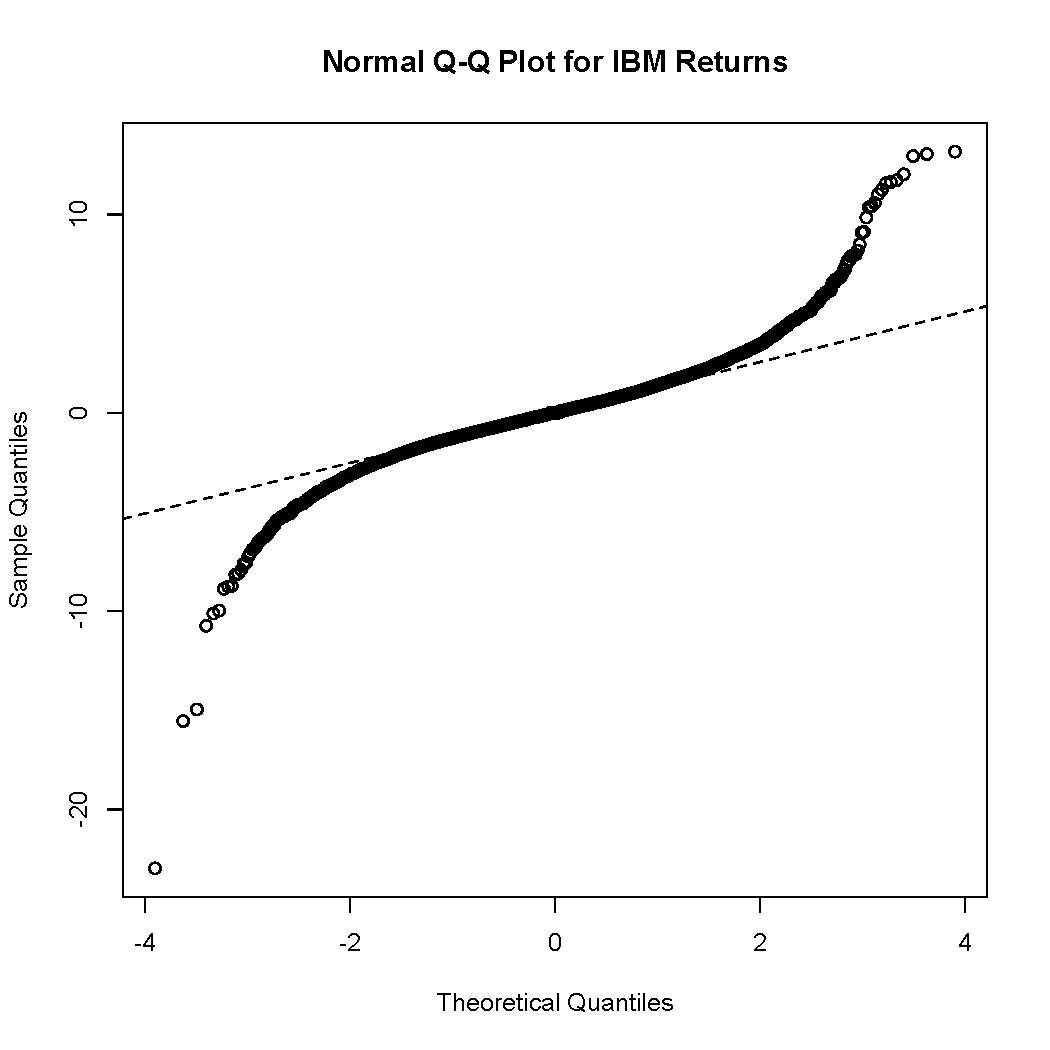
\includegraphics[scale=.6]{ibm-qq}
  \caption[Q-Q Plot of Returns]{By looking at a quantile-quantile plot of our data set, we see that returns are not normally distributed. The tails deviate sharply from normality.}
  \label{figure:ibm-qq}
\end{figure}

\begin{verbatim}
rets<-read.table("d-ibmvwewsp6203")
attach(rets)
retsts<-ts(V2)
plot(retsts,ylab="Returns")

qqnorm(V2,main="Normal Q-Q Plot for IBM Returns")
qqline(V2,lty=2)

plot(rets[,1]/10000, ibm, ylab="IBM Returns", xlab="Year")
\end{verbatim}

\begin{figure}[tb]
  \centering
  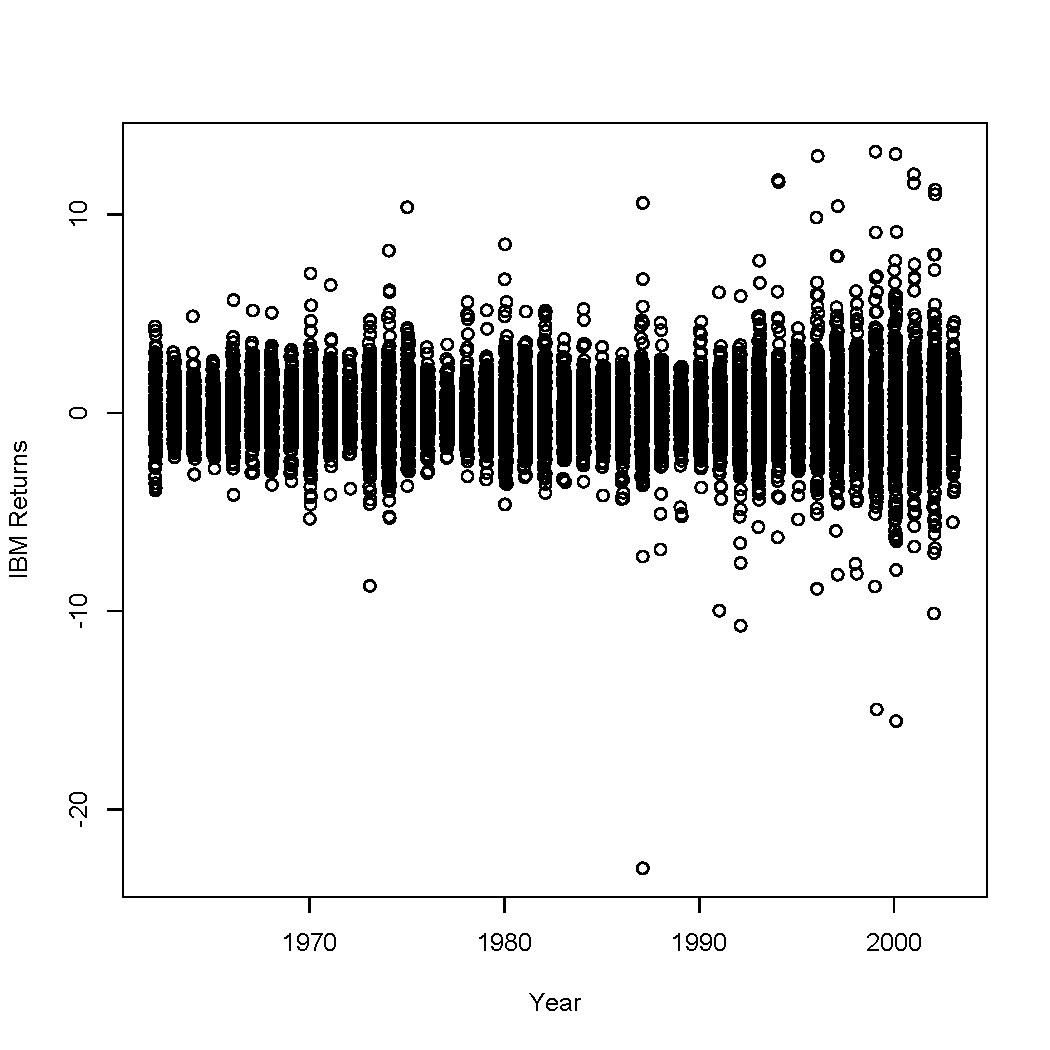
\includegraphics[scale=.6]{ibm-ret}
  \caption[IBM Returns]{IBM returns become more varied over time, deviating further from zero.}
  \label{figure:ibm-ret}
\end{figure}

\pagebreak
\paragraph{Normal Distribution.} For the sake of simplicity, returns are often considered to be \emph{\mbox{normally} distributed}. However, the lower bound of a simple is -1, total loss of the asset. The normal distribution has no lower bound. Also, multiperiod returns (\emph{the product of one-period \mbox{returns}, \eqref{eq:multiperiod} is a multiperiod return}) of a normally distributed returns are themselves not normally distributed. Additionally, asset returns observed in reality have positive excess kurtosis, and do not fit the normal distribution.

\paragraph{Lognormal Distribution.} Instead of assuming a normal distribution, we could assume that the log returns $r_t$ of an asset are independent and identically distributed (\emph{iid}) as normal with mean $\mu$ and variance $\sigma^2$, which makes simple returns iid lognormal random variables, and mean and variance are,
\[
E(R_t)=\exp \left( \mu + \frac{\sigma^2}{2} \right) -1, \quad
\text{Var}(R_t) = \exp(2\mu+\sigma^2)[\exp(\sigma^2)-1].
\]
The mean and variance of the log returns $r_t$ when $m_1$ and $m_2$ are the mean and variance of the simple return $R_t$
\[
E(r_t) = \ln \left( \frac{m_1+1}{\sqrt{1+m_2 / (1+m_1)^2}} \right), \quad
\text{Var}(r_t)=\ln \left( 1+\frac{m_2}{(1+m_1)^2} \right).
\]

%$Y$ is lognormal if $X = \ln(Y)$ is normal.
